\documentclass{report}
\usepackage[T1]{fontenc} % Fontes T1
\usepackage[utf8]{inputenc} % Input UTF8
\usepackage[backend=biber, style=ieee]{biblatex} % para usar bibliografia
\usepackage{csquotes}
\usepackage[portuguese]{babel} %Usar língua portuguesa
\usepackage{blindtext} % Gerar texto automaticamente
\usepackage[printonlyused]{acronym}
\usepackage{hyperref} % para autoref
\usepackage{graphicx}
\usepackage{booktabs}
\usepackage{float}
\usepackage{listings}
\usepackage{color}

\definecolor{dkgreen}{rgb}{0,0.6,0}
\definecolor{gray}{rgb}{0.5,0.5,0.5}
\definecolor{mauve}{rgb}{0.58,0,0.82}

\lstset{frame=tb,
  language=Python,
  aboveskip=3mm,
  belowskip=3mm,
  showstringspaces=false,
  columns=flexible,
  basicstyle={\small\ttfamily},
  numbers=none,
  numberstyle=\tiny\color{gray},
  keywordstyle=\color{blue},
  commentstyle=\color{dkgreen},
  stringstyle=\color{mauve},
  breaklines=true,
  breakatwhitespace=true,
  tabsize=3,
}

\graphicspath{ {./ss/} }

\bibliography{bibliografia}


\begin{document}
%%
% Definições
%
\def\titulo{Speedtest em Python}
\def\data{23 de Abril de 2019}
\def\autores{José Vasco Carvalho de Sousa, José Luís Rodrigues Costa,}
\def\autorescontactos{(93049) jvcs@ua.pt, (92996) joselcosta@ua.pt}
\def\versao{1.0}
\def\departamento{Departamento de Eletrónica Telecomunicações e Informática}
\def\empresa{Universidade de Aveiro}
\def\logotipo{ua.pdf}
%
%%%%%% CAPA %%%%%%
%
\begin{titlepage}

\begin{center}
%
\vspace*{50mm}
%
{\Huge \titulo}\\ 
%
\vspace{10mm}
%
{\Large \empresa}\\
%
\vspace{10mm}
%
{\LARGE \autores}\\ 
%
\vspace{30mm}
%
\begin{figure}[h]
\center
\includegraphics{\logotipo}
\end{figure}
%
\vspace{30mm}
\end{center}
%
\begin{flushright}
\versao
\end{flushright}
\end{titlepage}

%%  Página de Título %%
\title{%
{\Huge\textbf{\titulo}}\\
{\Large \departamento\\ \empresa}
}
%
\author{%
    \autores \\
    \autorescontactos
}
%
\date{\data}
%
\maketitle

\pagenumbering{roman}

%%%%%% RESUMO %%%%%%
\begin{abstract}
\par Este relatório aborda a motivação, a implementação e apresenta testes que comprovam o funcionamento correto do programa Speedtest, desenvolvido em Python\cite{python},
\par Atualmente, a largura de banda\cite{brandwidth} e a latência\cite{ping} são dois dos principais fatores que levam os clientes a escolher uma determinada operadora de telecomunicações.
\par Com efeito de avaliar estes dois fatores, existem diversos programas que calculam de uma forma mais ou menos precisa ambos.
\par Este programa faz essas avaliações utilizando sockets e o protocolo TCP\cite{tcp}.
De uma forma sucinta, para o teste de latência o programa começa por registar o tempo atual, de seguida envia uma mensagem ao servidor, recebe a resposta e por fim regista novamente o tempo e faz a diferença
entre o tempo atual e o tempo anterior. No fim deste processo temos a lantência entre a nossa máquina e o servidor em \ac{ms}.
\par Para o teste de largura de banda o programa começa por registar o tempo atual, de seguida envia uma mensagem ao servidor, recebe uma quantidade x Mb de dados e por fim regista novamente o tempo,
faz a diferença entre o tempo atual e o tempo anterior e faz também a devisão pela quantidade x Mb. No fim deste processo temos a velocidade de download em \ac{mbs}.
\end{abstract}

    
\tableofcontents
% \listoftables     % descomentar se necessário
% \listoffigures    % descomentar se necessário


%%%%%%%%%%%%%%%%%%%%%%%%%%%%%%%
\clearpage
\pagenumbering{arabic}

%%%%%%%%%%%%%%%%%%%%%%%%%%%%%%%%
\chapter{Introdução}
\label{chap.introducao}

\par Este relatório aborda a motivação, a implementação e apresenta testes que comprovam o funcionamento correto do programa Speedtest, desenvolvido em Python\cite{python},
\par Este relatório está dividido em quatro capítulos.
Depois desta introdução,
no \autoref{chap.metodologia} é apresentada a metodologia seguida,
no \autoref{chap.testes} são apresentados testes de depuração,
no \autoref{chap.resultados} são apresentados os resultados obtidos,
Finalmente, no \autoref{chap.conclusao} são apresentadas
as conclusões do relatório.

\chapter{Metodologia}
\label{chap.metodologia}

\section{Linguagem}
\par O programa Speedtest foi desenvolvido na linguagem de programação Python\cite{python}, sendo utilizada a versão 3.7
Esta linguagem é uma linguagem de alto nível desenvolvida pela comunidade e gerida pela organização Python Software Fundation\cite{pythonorg}.
\par Nos dias de hoje esta linguagem é bastante popular, sobretudo na área da inteligência artifical.
\section{Código}

\subsection{Bibliotecas Utilizadas}
\par Para facilitar a implementação de certas funcionalidades deste programa foram utilizadas as seguintes bibliotecas.
\begin{lstlisting}[escapeinside={(*}{*)}]
    import socket
    import time
    import random
    import datetime
    import sys
    import json
    import csv
    import hashlib
    from Crypto.PublicKey import RSA
    from Crypto.Hash import SHA256
    from Crypto.Signature import PKCS1_v1_5
\end{lstlisting}

\subsection{Validação dos Argumentos}
\par Com o objetivo de validar os argumentos fornecidos pelo utilizador, foi implementado um algorítmo de validação
\par Em primeiro lugar esse algorítmo verifica se o número de argumentos fornecidos corresponde ao número de argumentos necessário para o correcto funcionamento do programa.
\par Por fim o algorítmo verifica se os argumentos interval (tempo que decorre entre dois testes realizados), num (número de testes a serem realizados) e [country or id] 
(nome do país do servidor ou identificador do servidor), são números positivos nos dois primeiros casos e número ou string no terceiro.
\par Caso estas duas condições não sejam verificadas, o programa não corre e mostra uma mensagem de erro.
\begin{lstlisting}[escapeinside={(*}{*)}]
#Verificar validade dos argumentos
def checkArguments():
    if len(sys.argv) < 4:
        print("Ajuda: python3 client.py interval num [country or id]")
        sys.exit(0)

    if not sys.argv[1].isdigit() and int(sys.argv[1]) > 0:
        print("Erro: argumento 'interval' tem um formato incorreto")
        sys.exit(0)

    if not sys.argv[2].isdigit() and int(sys.argv[2]) > 0:
        print("Erro: argumento 'num' tem um formato incorreto")
        sys.exit(0)

    if not (sys.argv[3].isnumeric() or sys.argv[3].isalpha()):
        print("Erro: argumento 'country or id' tem um formato incorreto")
        sys.exit(0)
\end{lstlisting}

\subsection{Escolha do Servidor}
\par Para efetuar a escolha do servidor que serve para efetuar os testes, o programa tem dois métodos que possibilitam esta escolha
\par Em primeiro lugar o programa converte o conteúdo do ficheiro servers.json num objecto JSON.
\par De seguida o algorítmo verifica se o último argumento é um ID (número) ou um nome de um país (string).
\par Caso seja um ID, é feita a iteração do objeto JSON e quando é encontrado o servidor com o ID correspondente ao ID fornecido no argumento, é escolhido esse mesmo servidor.
\par Caso seja um país, é feita a iteração do objeto JSON e quando é encontrado um servidor com o país correspondente ao país fornecido no argumento, este é armazenado num novo array.
De seguida é gerado um número aleatório que servirá como indíce do novo array, que contém todos os servidores de um determinado país.

\begin{lstlisting}[escapeinside={(*}{*)}]
    #Le o ficheiro servers.json e retorna-o como um objecto JSON 
    def loadServers():
        with open('servers.json') as f:
            data = json.load(f)
            return data
    
    #Seleciona um servidor tendo em conta o argumento fornecido
    def selectServer(arg):
        allServers = loadServers()
    
    
        if arg.isalpha():
            targetCountryServers = []
            i = 0
    
            #Caso o nome do pais inclua espacos como por exemplo United States
            if(len(sys.argv) > 4):
                for i in range(4, len(sys.argv)):
                    arg += " " + sys.argv[i]
                
            #Caso o argumento seja um nome de um pais (alphanum)
            for server in allServers["servers"]:
                    if server["country"].lower() == arg.lower():
                        targetCountryServers.append(server)
                        i += 1
            
            #Verificar se o array com os possiveis servidores esta vazio
            if len(targetCountryServers) == 0:
                print("Erro: Nao existe nenhum servidor localizado no pais fornecido")
                sys.exit(0)
            else:
                k = random.randint(0,(i - 1)) 
                return targetCountryServers[k]["host"].split(":")
        
    
        #Caso o argumento seja um ID (digit)
        elif arg.isnumeric():
            for server in allServers["servers"]:
                    
                    if server["id"] == int(arg):
                        return server["host"].split(":")
            
            #Caso nao seja encontrado nenhum servidor com um id correspondente
            print("Erro: Nao existe nenhum servidor com o id fornecido")
            sys.exit(0)
    
        else:
            print("Erro: Nao foi encontrado nenhum servidor")
            sys.exit(0)
\end{lstlisting}

\subsection{Teste de Latência}
\par Com o objetivo de realizar o teste de latência o programa começa por criar um socket, conectando-se ao servidor previamente escolhido.
\par De seguida é enviado um comando para esse servidor pelo protocolo TCP\cite{tcp}, de seguida o servidor envia uma resposta com o timestamp atual.
Por fim o programa regista novamente o tempo e faz a diferença entre o tempo atual e o tempo anteriormente registado. O resultado é a latência entre a máquina e o servidor em \ac{ms}.
\begin{lstlisting}
#Faz o teste de ping ao host fornecido
def ping(host, port):
    i = 0
    totalPing = 0
    print("> Tesde de latencia iniciado < \n")

    while i < 10:
        #Cria o socket do tipo tcp
        client = socket.socket(socket.AF_INET, socket.SOCK_STREAM)

        #O tempo maximo de espera por ligacao ao servidor e 10 segundos
        client.settimeout(10)

        #Tenta a ligacao ao servidor, caso falhe uma mensagem e mostrada e o valor de ping e -1
        try:
            client.connect((host,port))

        except socket.timeout:
            print("Erro: Impossivel conectar ao servidor")
            return -1 
         
        #Tempo em milisegundos antes de enviar o comando
        timeBefore = time.time() * 1000

        #Envio do comando para o servidor atraves de TCP
        client.send(("PING " + str(timeBefore) + "\n").encode("utf-8"))
        
        #Resposta do servidor
        response = client.recv(1024)

        #Tempo em milisegundos depois de receber a resposta do servidor
        timeAfter = time.time() * 1000

        #Fecha a conexao ao servidor
        client.close()

        #Mostra resposta do servidor    
        print(response)

        #Delta do tempo, da a latencia em milisegundos
        deltaTime = timeAfter - timeBefore

        totalPing += deltaTime
        print("Latencia para " + str(host) + " e de " + str(round(deltaTime)) + "ms")
        i += 1
        time.sleep(2)

    print("\n")

    #Retorna o valor medio do ping
    return round(totalPing/10)

#Mostra resposta do servidor ao comando "HI \n"
def hello(host, port):
    #Cria o socket do tipo tcp
    client = socket.socket(socket.AF_INET, socket.SOCK_STREAM)

    #Tempo maximo de espera por resposta do socket (10 segundos)
    client.settimeout(10)

    #Tenta a ligacao ao servidor, caso falhe uma mensagem e mostrada
    try:
        client.connect((host,port))

    except socket.timeout:
        print("Erro: Impossivel conectar ao servidor")

    #Envia o comando para o servidor    
    client.send(("HI\n").encode("utf-8"))

    #Recebe a resposta do servidor
    response = client.recv(4096).decode('utf-8')

    #Mostra a resposta
    print(response)

    #Fecha a conexao com o servidor
    client.close()

\end{lstlisting}

\subsection{Teste de largura de banda}
\par Com o objetivo de realizar o teste de largura de banda o programa começa por criar um socket, conectando-se ao servidor previamente escolhido.
Depois desta etapa, o programa regista o tempo atual, de seguida é enviado um comando para esse servidor pelo protocolo TCP\cite{tcp}, 
o servidor envia uma resposta com um tamanho aleatório entre 10Mb e 100Mb. Dentro de um ciclo infinito while, é lida a resposta enviada até que passem 10 segundos, neste caso 
o valor de download total em Mb é atualizado para o valor que realmente foi baixado, ou então até que o servidor 
deixe de enviar dados (fim do download). Quando uma destas condições é atingida o ciclo para e é registado novamente o tempo atual. Para efeitos de teste o conteúdo enviado pelo servidor
é armazenado num ficheiro de texto.
\par A largura de banda é obtida com a divisão do download total em Mb e o tempo passado em segundos. Daí resulta a largura de banda em \ac{mbs}.
Por fim o programa regista novamente o tempo e faz a diferença entre o tempo atual e o tempo anteriormente registado. O resultado é a latência entre a máquina e o servidor em \ac{ms}.
\begin{lstlisting}
    #Faz o teste de ping ao host fornecido
def ping(host, port):
    i = 0
    totalPing = 0
    print("> Tesde de latencia iniciado < \n")

    while i < 10:
        #Cria o socket do tipo tcp
        client = socket.socket(socket.AF_INET, socket.SOCK_STREAM)

        #O tempo maximo de espera por ligacao ao servidor e 10 segundos
        client.settimeout(10)

        #Tenta a ligacao ao servidor, caso falhe uma mensagem e mostrada e o valor de ping e -1
        try:
            client.connect((host,port))

        except socket.timeout:
            print("Erro: Impossivel conectar ao servidor")
            return -1 
         
        #Tempo em milisegundos antes de enviar o comando
        timeBefore = time.time() * 1000

        #Envio do comando para o servidor atraves de TCP
        client.send(("PING " + str(timeBefore) + "\n").encode("utf-8"))
        
        #Resposta do servidor
        response = client.recv(1024)

        #Tempo em milisegundos depois de receber a resposta do servidor
        timeAfter = time.time() * 1000

        #Fecha a conexao ao servidor
        client.close()

        #Mostra resposta do servidor    
        print(response)

        #Delta do tempo, da a latencia em milisegundos
        deltaTime = timeAfter - timeBefore

        totalPing += deltaTime
        print("Latencia para " + str(host) + " e de " + str(round(deltaTime)) + "ms")
        i += 1
        time.sleep(2)

    print("\n")

    #Retorna o valor medio do ping
    return round(totalPing/10)

#Mostra resposta do servidor ao comando "HI \n"
def hello(host, port):
    #Cria o socket do tipo tcp
    client = socket.socket(socket.AF_INET, socket.SOCK_STREAM)

    #Tempo maximo de espera por resposta do socket (10 segundos)
    client.settimeout(10)

    #Tenta a ligacao ao servidor, caso falhe uma mensagem e mostrada
    try:
        client.connect((host,port))

    except socket.timeout:
        print("Erro: Impossivel conectar ao servidor")

    #Envia o comando para o servidor    
    client.send(("HI\n").encode("utf-8"))

    #Recebe a resposta do servidor
    response = client.recv(4096).decode('utf-8')

    #Mostra a resposta
    print(response)

    #Fecha a conexao com o servidor
    client.close()

\end{lstlisting}

\subsection{Escrita dos resultados num ficheiro CSV}
\par Para efetuar a escrita dos resultados obtidos num ficheiro CSV o programa começa por criar um novo ficheiro denominado como report.csv
De seguida são escritos os cabeçalhos ['counter', 'id', 'data', 'latency', 'bandwidth', 'check'] e depois as linhas com os valores obtidos com as funções previamente apresentadas.
\begin{lstlisting}
#Iniciar o ficheiro para escrita / fazer testes

with open('report.csv', mode='w') as csv_file:
        fieldnames = ['counter', 'id', 'data', 'latency', 'bandwidth', 'check']

        #Escrever os cabecalhos
        writer = csv.DictWriter(csv_file, fieldnames=fieldnames)
        writer.writeheader()

        while True:
            serverData = selectServer(str(sys.argv[3]))
            curPing = ping(serverData[0], int(serverData[1]))
            curDownload = download(serverData[0], int(serverData[1]))

            numTests -= 1

            print("Resultados | Ping -> " + str(curPing) + "ms - Download -> " + str(curDownload) + "Mb/s")
            print("Info: Teste realizado com sucesso, faltam  " + str(numTests) + " para terminar\n")
            
            #escrever as linhas
            writer.writerow({'counter': str(numTests) , 'id': str(matchHost(serverData[0] + ':' + serverData[1])), 'data': str(datetime.datetime.now().isoformat()), 'latency': str(curPing), 'bandwidth': str(curDownload), 'check': str(numTests) + str(matchHost(serverData[0] + ':' + serverData[1])) + str(datetime.datetime.now().isoformat()) + str(curPing) + str(curDownload) })
\end{lstlisting}

\subsection{Assinatura do ficheiro CSV}
\par Com o objetivo de assinar o ficheiro CSV com uma chave privada, o programa começa por ler uma chave privada RSA denominada por key.priv.pem e faz a assinatura digital do ficheiro
report.csv linha a linha, e por fim escreve o resultado num ficheiro denominado por report.sig.
\begin{lstlisting}
def signReport():
privkey = RSA.importKey(open('key.priv.pem', 'r').read())
signer = PKCS1_v1_5.new(privkey)
unsigned_file = open('report.csv', 'r')
signed_file = open('report.sig', 'wb')
line = unsigned_file.readline()

for line in unsigned_file:
    h = SHA256.new(line.encode('utf-8'))
    signed_line = signer.sign(h)
    signed_file.write(signed_line)
    line = unsigned_file.readline()
\end{lstlisting}

\chapter{Testes de Depuração}
\label{chap.testes}
\section{Argumentos}
\begin{figure}[h!]
    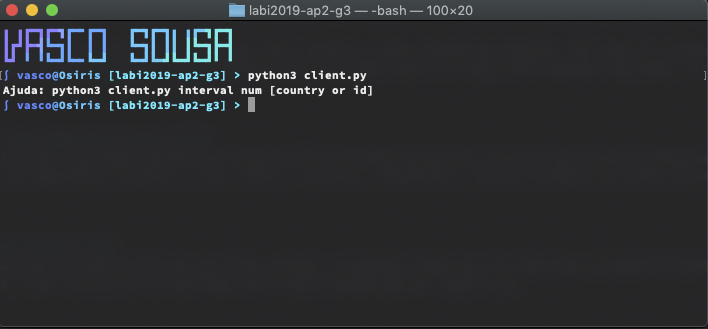
\includegraphics[width=\linewidth]{ss1.jpg}
    \caption{Output do programa quando se executa o mesmo sem fornecer argumentos }
    \label{fig:noarguments}
\end{figure}
\begin{figure}[h!]
    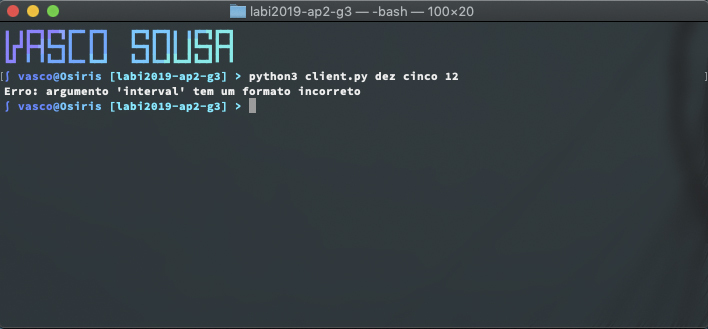
\includegraphics[width=\linewidth]{ss2.jpg}
    \caption{Output do programa quando se executa o mesmo fornecendo argumentos com o formato errado }
    \label{fig:wrongarguments}
\end{figure}

\newpage
\section{Conexão ao servidor}
\begin{figure}[h!]
    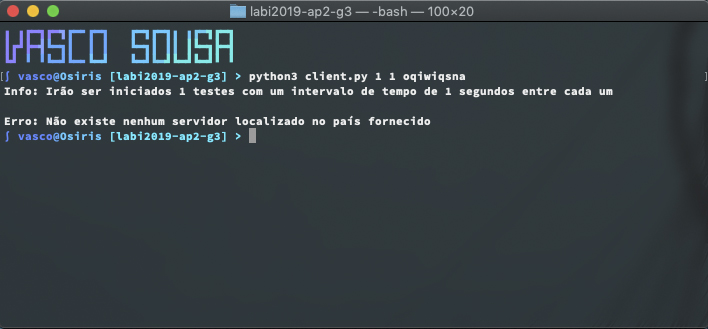
\includegraphics[width=\linewidth]{ss3.jpg}
    \caption{Output do programa quando se executa o mesmo fornecendo um país em que não existem servidores }
    \label{fig:wrongcountry}
\end{figure}

\begin{figure}[h!]
    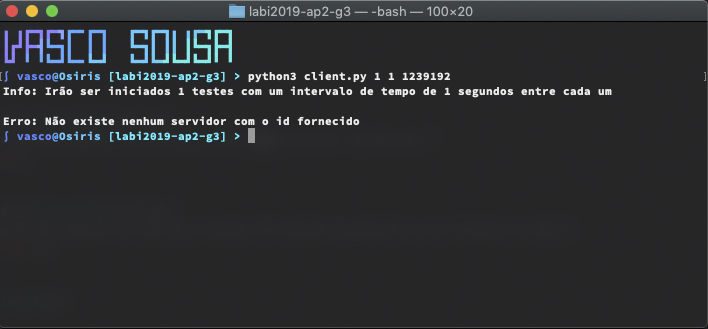
\includegraphics[width=\linewidth]{ss5.jpg}
    \caption{Output do programa quando se executa o mesmo fornecendo um id que não responde a nenhum servidor }
    \label{fig:wrongcountry}
\end{figure}

\begin{figure}[h!]
    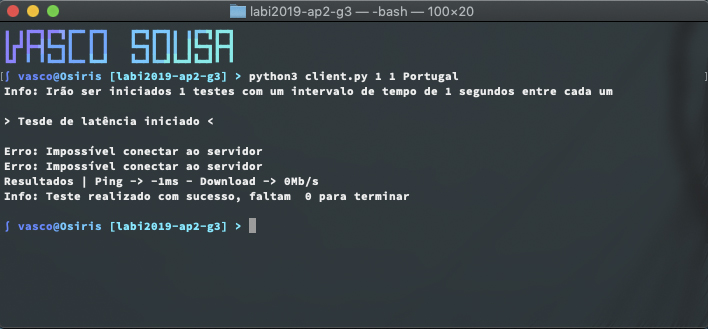
\includegraphics[width=\linewidth]{ss4.jpg}
    \caption{Output do programa quando se executa o mesmo sem conexão à internet ou quando não é possível conectar com o servidor }
    \label{fig:noconnection}
\end{figure}

\newpage
\section{Escrita do Ficheiro CSV}
\begin{figure}[h!]
    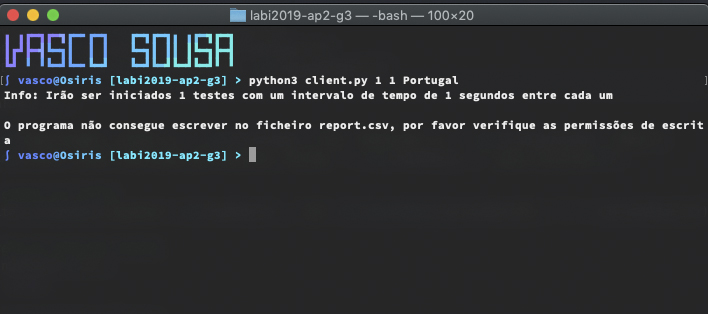
\includegraphics[width=\linewidth]{ss8.jpg}
    \caption{Output do programa quando se executa o mesmo e não existem permissões para criar e escrever no ficheiro report.csv }
    \label{fig:noconnection}
\end{figure}

\newpage
\section{Assinatura Digital}
\begin{figure}[h!]
    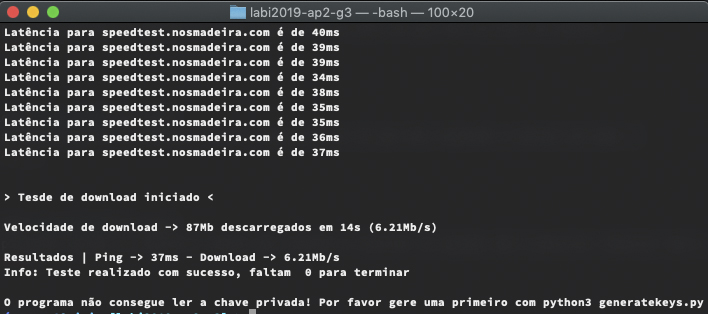
\includegraphics[width=\linewidth]{ss7.jpg}
    \caption{Output do programa quando se executa o mesmo e não existe um ficheiro key.priv.pem para ser utilizado ou não existem permissões para abrir esse mesmo ficheiro, para assinar digitalmente o report.csv }
    \label{fig:noconnection}
\end{figure}

\chapter{Resultados}
\label{chap.resultados}
\par Para testar o bom funcionamento do programa, foram feitos dez testes espaçados de dez segundos numa conexão à internet fibra de uma empresa de telecomunicações portuguesa.
\par Cinco destes testes foram feitos em servidores localizados em Portugal, os outros cinco foram realizados em servidores localizados na China.
\begin{table}[h!]
    \begin{tabular}{|c|c|c|c|c|}
    \hline
    \textbf{Counter} & \textbf{Id} & \textbf{Date}              & \textbf{\begin{tabular}[c]{@{}c@{}}Latency  \\ (ms)\end{tabular}} & \textbf{Bandwidth (mb/s)} \\ \hline
    4                & 1758        & 2019-04-24T10:46:35.893562 & 19                                                                & 4.38                      \\ \hline
    3                & 1249        & 2019-04-24T10:47:36.168147 & 47                                                                & 4.40                      \\ \hline
    2                & 19253       & 2019-04-24T10:48:28.458914 & 27                                                                & 4.21                      \\ \hline
    1                & 1249        & 2019-04-24T10:49:19.441649 & 19                                                                & 5.28                      \\ \hline
    0                & 9729        & 2019-04-24T10:50:07.572682 & 21                                                                & 5.77                      \\ \hline
    \end{tabular}
    \caption{Resultados dos testes realizados em servidores portugueses}
\end{table}

\begin{table}[h!]
    \begin{tabular}{|c|c|c|c|c|}
    \hline
    \textbf{Counter} & \textbf{Id} & \textbf{Date}              & \textbf{\begin{tabular}[c]{@{}c@{}}Latency  \\ (ms)\end{tabular}} & \textbf{Bandwidth (mb/s)} \\ \hline
    4                & 21584       & 2019-04-24T10:55:01.546779 & 322                                                               & 1.02                      \\ \hline
    3                & 17228       & 2019-04-24T10:56:36.157917 & 345                                                               & 0.90                      \\ \hline
    2                & 17222       & 2019-04-24T10:57:18.259643 & 321                                                               & 0.89                      \\ \hline
    1                & 17437       & 2019-04-24T10:58:09.124659 & 310                                                               & 0.89                      \\ \hline
    0                & 9484        & 2019-04-24T10:59:12.772322 & 384                                                               & 0.90                      \\ \hline
    \end{tabular}
    \caption{Resultados dos testes realizados em servidores chineses}
\end{table}

\par Comparando os resultados obtidos, podemos concluir que quanto mais próximo os servidores estão físicamente da nossa máquina, menor a latência e menor também a largura de banda,
como seria de esperar.
\par Apesar destes resultados serem bastante próximos da realidade, existem fatores, que podem ter influência nos resultados finais, que o programa speedtest não tem em conta.

\chapter{Conclusões}
\label{chap.conclusao}
\par Concluindo, este projeto utiliza todas as técnicas lecionadas no segundo semestre do primeiro ano da Unidade Curricular de Laboratórios de Informática para a realização de um Speedtest desenvolvido em Python\cite{python}, com toda a funcionalidade proposta e com toda a documentação necessária. 
\par Foram também feitos os testes de depuração necessário para avaliar o bom funcionamento do programa.
\par Os resultados de latência e download são influênciados pela distância física da máquina ao servidor de teste, como era de esperar.
\par Salientamos
que os resultados deste Speedtest tanto na latência, como na largura de banda aproximam os valores reais, mas não são totalmente precisos devido a influências de pequenos fatores como o "slow start" do protocolo TCP.

\chapter*{Contribuições dos autores}
\par Para a realização deste trabalho, ambos os autores desenvolveram o código dos ficheiros .py, sendo que Vasco Sousa teve uma maior influência no desenvolvimento dos métodos envolvidos no cálculo da latência, da largura de banda
e seleção de servidor. Já Luis Costa foi o principal responsável nos métodos responsáveis por ler a chave RSA, assinar digitalmente o ficheiro report.csv e escrever no ficheiro report.csv.
\par Apesar de o desenvolvimento do programa ter sido distribuído pelos dois autores, o desenvolvimento foi mútuo e partilhado pelos mesmos.
\par Ambos os autores contribuíram para a escrita de cada um dos capítulos deste documento.
\par De uma forma geral, as contruibuições dos autores são de 50\% de Vasco Sousa e 50\% para Luis Costa.


%%%%%%%%%%%%%%%%%%%%%%%%%%%%%%%%%
\chapter*{Acrónimos}
\begin{acronym}
\acro{ua}[UA]{Universidade de Aveiro}
\acro{ms}[ms]{milissegundos}
\acro{mbs}[mb/s]{mb/s}
\end{acronym}


%%%%%%%%%%%%%%%%%%%%%%%%%%%%%%%%%
\printbibliography

\end{document}
